% \section{Methodology: A Hybrid YOLO-MobileNet Architecture for Edge Inference}
% \label{sec:yolo_mobilenet}

% Deploying deep learning–based object detection on resource-constrained edge devices requires a careful balance between detection accuracy, computational efficiency, and system-level compatibility. To address these constraints, the proposed methodology adopts a hybrid design that combines a modern YOLO detection head with a lightweight MobileNetV4 backbone and an optimized on-device inference runtime. The following subsections describe the selected detection architecture, the rationale for choosing MobileNetV4 as the backbone, the inference optimization using LiteRT, and the practical integration of the proposed model into the YOLO framework for efficient edge deployment.

% \subsection{YOLOv11 Model}
% The YOLO framework, pioneered by Joseph Redmon, revolutionized real-time object detection by introducing a grid-based approach to predict bounding boxes and class probabilities simultaneously This innovative design facilitates a highly efficient detection process, making YOLO particularly suitable for applications needing real-time performance. \cite{ali_2024_the}

% To achieve high-efficiency object detection, the YOLO architecture operates by partitioning an input image into a grid. Unlike multi-stage detectors, it extracts features via a deep Convolutional Neural Network (CNN) to predict bounding boxes and class probabilities simultaneously. To accommodate objects of varying sizes, the model utilizes anchor boxes at multiple scales, while the final output is refined through Non-Maximum Suppression (NMS) to eliminate redundant, low-confidence predictions.

% Released in 2024, YOLO11 is the latest version to date, built upon YOLOv8 with structural improvements and parameter optimization that achieve enhanced detection performance \cite{ultralytics_2024_yolo11}. In particular, it increases applicability in areas such as pose estimation, orientation detection, classification tasks, and instance segmentation, thereby expanding its utility across diverse computer vision applications.

% \begin{figure}[htbp]
%     \centering
%     \resizebox{\columnwidth}{!}{%
%     \begin{tikzpicture}[
%         node distance=0.4cm and 0.8cm,
%         font=\sffamily\bfseries\small,
%         module/.style={
%             draw=cyan!60, fill=cyan!10, rounded corners, drop shadow,
%             minimum width=2.0cm, minimum height=0.8cm, align=center, line width=0.8pt, font=\scriptsize\sffamily\bfseries
%         },
%         yolo/.style={
%             draw=orange!60, fill=orange!10, rounded corners, drop shadow,
%             minimum width=2.2cm, minimum height=4.6cm, align=center, font=\sffamily\bfseries\normalsize
%         },
%         task/.style={
%             draw=green!60!black, fill=green!10, rounded corners, drop shadow,
%             minimum width=3.0cm, minimum height=0.6cm, align=center, anchor=west, line width=0.8pt, font=\scriptsize\sffamily\bfseries
%         },
%         line/.style={draw=gray!60, line width=1pt},
%         arrow/.style={line, -{Stealth[scale=1.0]}}
%     ]

%     % Central YOLOv11 block
%     \node[yolo] (yolo11) {YOLO11};

%     % Left-side modules (Three key modules)
%     % Position C2PSA to be aligned vertically with the center
%     \node[module, left=1.0cm of yolo11] (c2psa) {C2PSA};
%     \node[module, above=0.3cm of c2psa] (sppf) {SPPF};
%     \node[module, below=0.3cm of c2psa] (c3k2) {C3K2};

%     % Right-side tasks (6 tasks)
%     % Position the top task relative to the center, then stack others below
%     \node[task, right=1.0cm of yolo11, anchor=west, yshift=2.0cm] (od) {Object Detection};
%     \node[task, below=0.2cm of od] (is) {Instance Segmentation};
%     \node[task, below=0.2cm of is] (ic) {Image Classification};
%     \node[task, below=0.2cm of ic] (pe) {Pose Estimation};
%     \node[task, below=0.2cm of pe] (ood) {Oriented Object\\Detection};
%     \node[task, below=0.2cm of ood] (ot) {Object Tracking};

%     % Connections: Modules to YOLOv11
%     % Merge lines from the three modules
%     \coordinate (merge_x) at ($(c2psa.east)!0.5!(yolo11.west)$);
    
%     % Draw vertical bar connecting the top and bottom modules at merging x-coord
%     \draw[line] (sppf.east) -| (merge_x) |- (c3k2.east);
    
%     % Connect C2PSA to the merge point
%     \draw[line] (c2psa.east) -- (merge_x);
    
%     % Arrow from merge point to YOLOv11
%     % Since merge_x is a coordinate, we need the intersection with C2PSA's y-level
%     \draw[arrow] (merge_x |- c2psa.east) -- (yolo11.west);

%     % Connections: YOLOv11 to Tasks
%     % Draw arrows from the right edge of YOLOv11 to each task
%     \foreach \t in {od, is, ic, pe, ood, ot} {
%         \draw[arrow] (yolo11.east |- \t.west) -- (\t.west);
%     }

%     \end{tikzpicture}%
%     }
%     \caption{Key architectural modules in YOLO11.}
%     \label{fig:yolo11}
% \end{figure}

% Key improvements in YOLO11 include the introduction of the Cross-Stage Partial with Self Attention (C2PSA) module, as seen in Figure \ref{fig:yolo11}, which combines the benefits of cross-stage partial networks with self-attention mechanisms. This enables the model to capture contextual information more effectively across multiple layers, improving object detection accuracy, especially for small and colluded objects. Additionally, in YOLO11, the C2f block has been replaced by C3k2, a custom implementation of the CSP Bottleneck that uses two convolutions, unlike YOLOv8's use of one large convolution. This block uses a smaller kernel, retaining accuracy while improving efficiency and speed. \cite{jegham_2025_yolo}

% \subsection{MobileNetv4}
% MobileNetV4 is a lightweight Convolutional Neural Network (CNN) architecture proposed by Google in 2024 \cite{qin_2024_mobilenetv4}. It serves as the latest iteration of the MobileNet series and aims to further optimize the balance between computational efficiency and model performance on mobile and edge computing devices. This architecture continues the core philosophy of the MobileNet family regarding lightweight design, yet it significantly enhances image classification performance through structural innovations and improvements in training strategies. \cite{chen_2025_mobilenetgdr}

% We select MobileNetV4-Small as the backbone for YOLO11 due to its superior efficiency-accuracy trade-off compared to alternative architectures. As demonstrated in Figure \ref{fig:mnv4_benchmark}\cite{qin_2024_mobilenetv4}, MobileNetV4 consistently achieves Pareto optimality across a diverse range of hardware platforms, including CPUs, DSPs, GPUs, and TPUs. Specifically, the red curve representing MobileNetV4 demonstrates higher ImageNet-1k Top-1 accuracy at equivalent or lower latency compared to predecessors (MobileNetV1–V3) and competing hybrid models such as FastViT and MobileOne. For instance, on the Pixel 6 CPU and Samsung Galaxy S23 GPU, MobileNetV4 maintains a distinct performance advantage, delivering high accuracy with significantly reduced inference time, making it the ideal candidate for our resource-constrained application. 

% \begin{figure}[ht]
%     \centering
%     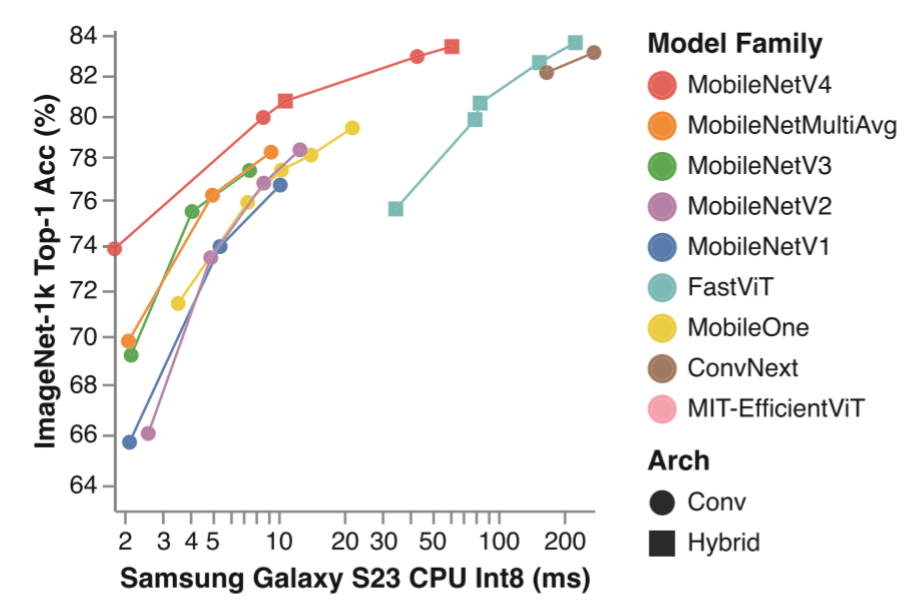
\includegraphics[width=1\linewidth]{Images/mnv4withothers.png}
%     \caption{MNv4 Models are Universally Mostly Pareto Optimal \cite{qin_2024_mobilenetv4}}
%     \label{fig:mnv4_benchmark}
% \end{figure}

% For instance, on the Pixel 6 CPU, MobileNetV4 achieves a Top-1 Accuracy of approximately 74\% with an ultra-low latency of just ~3 ms. In contrast, at the same 3 ms latency, the previous generation MobileNetV3 and MobileNetV2 only achieve approximately 66\% accuracy - a performance gap of nearly 8\%. Similarly, on the Samsung Galaxy S23 CPU, MobileNetV4 breaks the 80\% accuracy barrier at roughly 5 ms, a speed at which other efficient models like FastViT have not yet even started to register on the chart. This superior ``speed-vs-accuracy'' ratio makes MobileNetV4-Small uniquely suited for our real-time embedded CPU applications.

% \begin{figure}[ht]
%     \centering
%     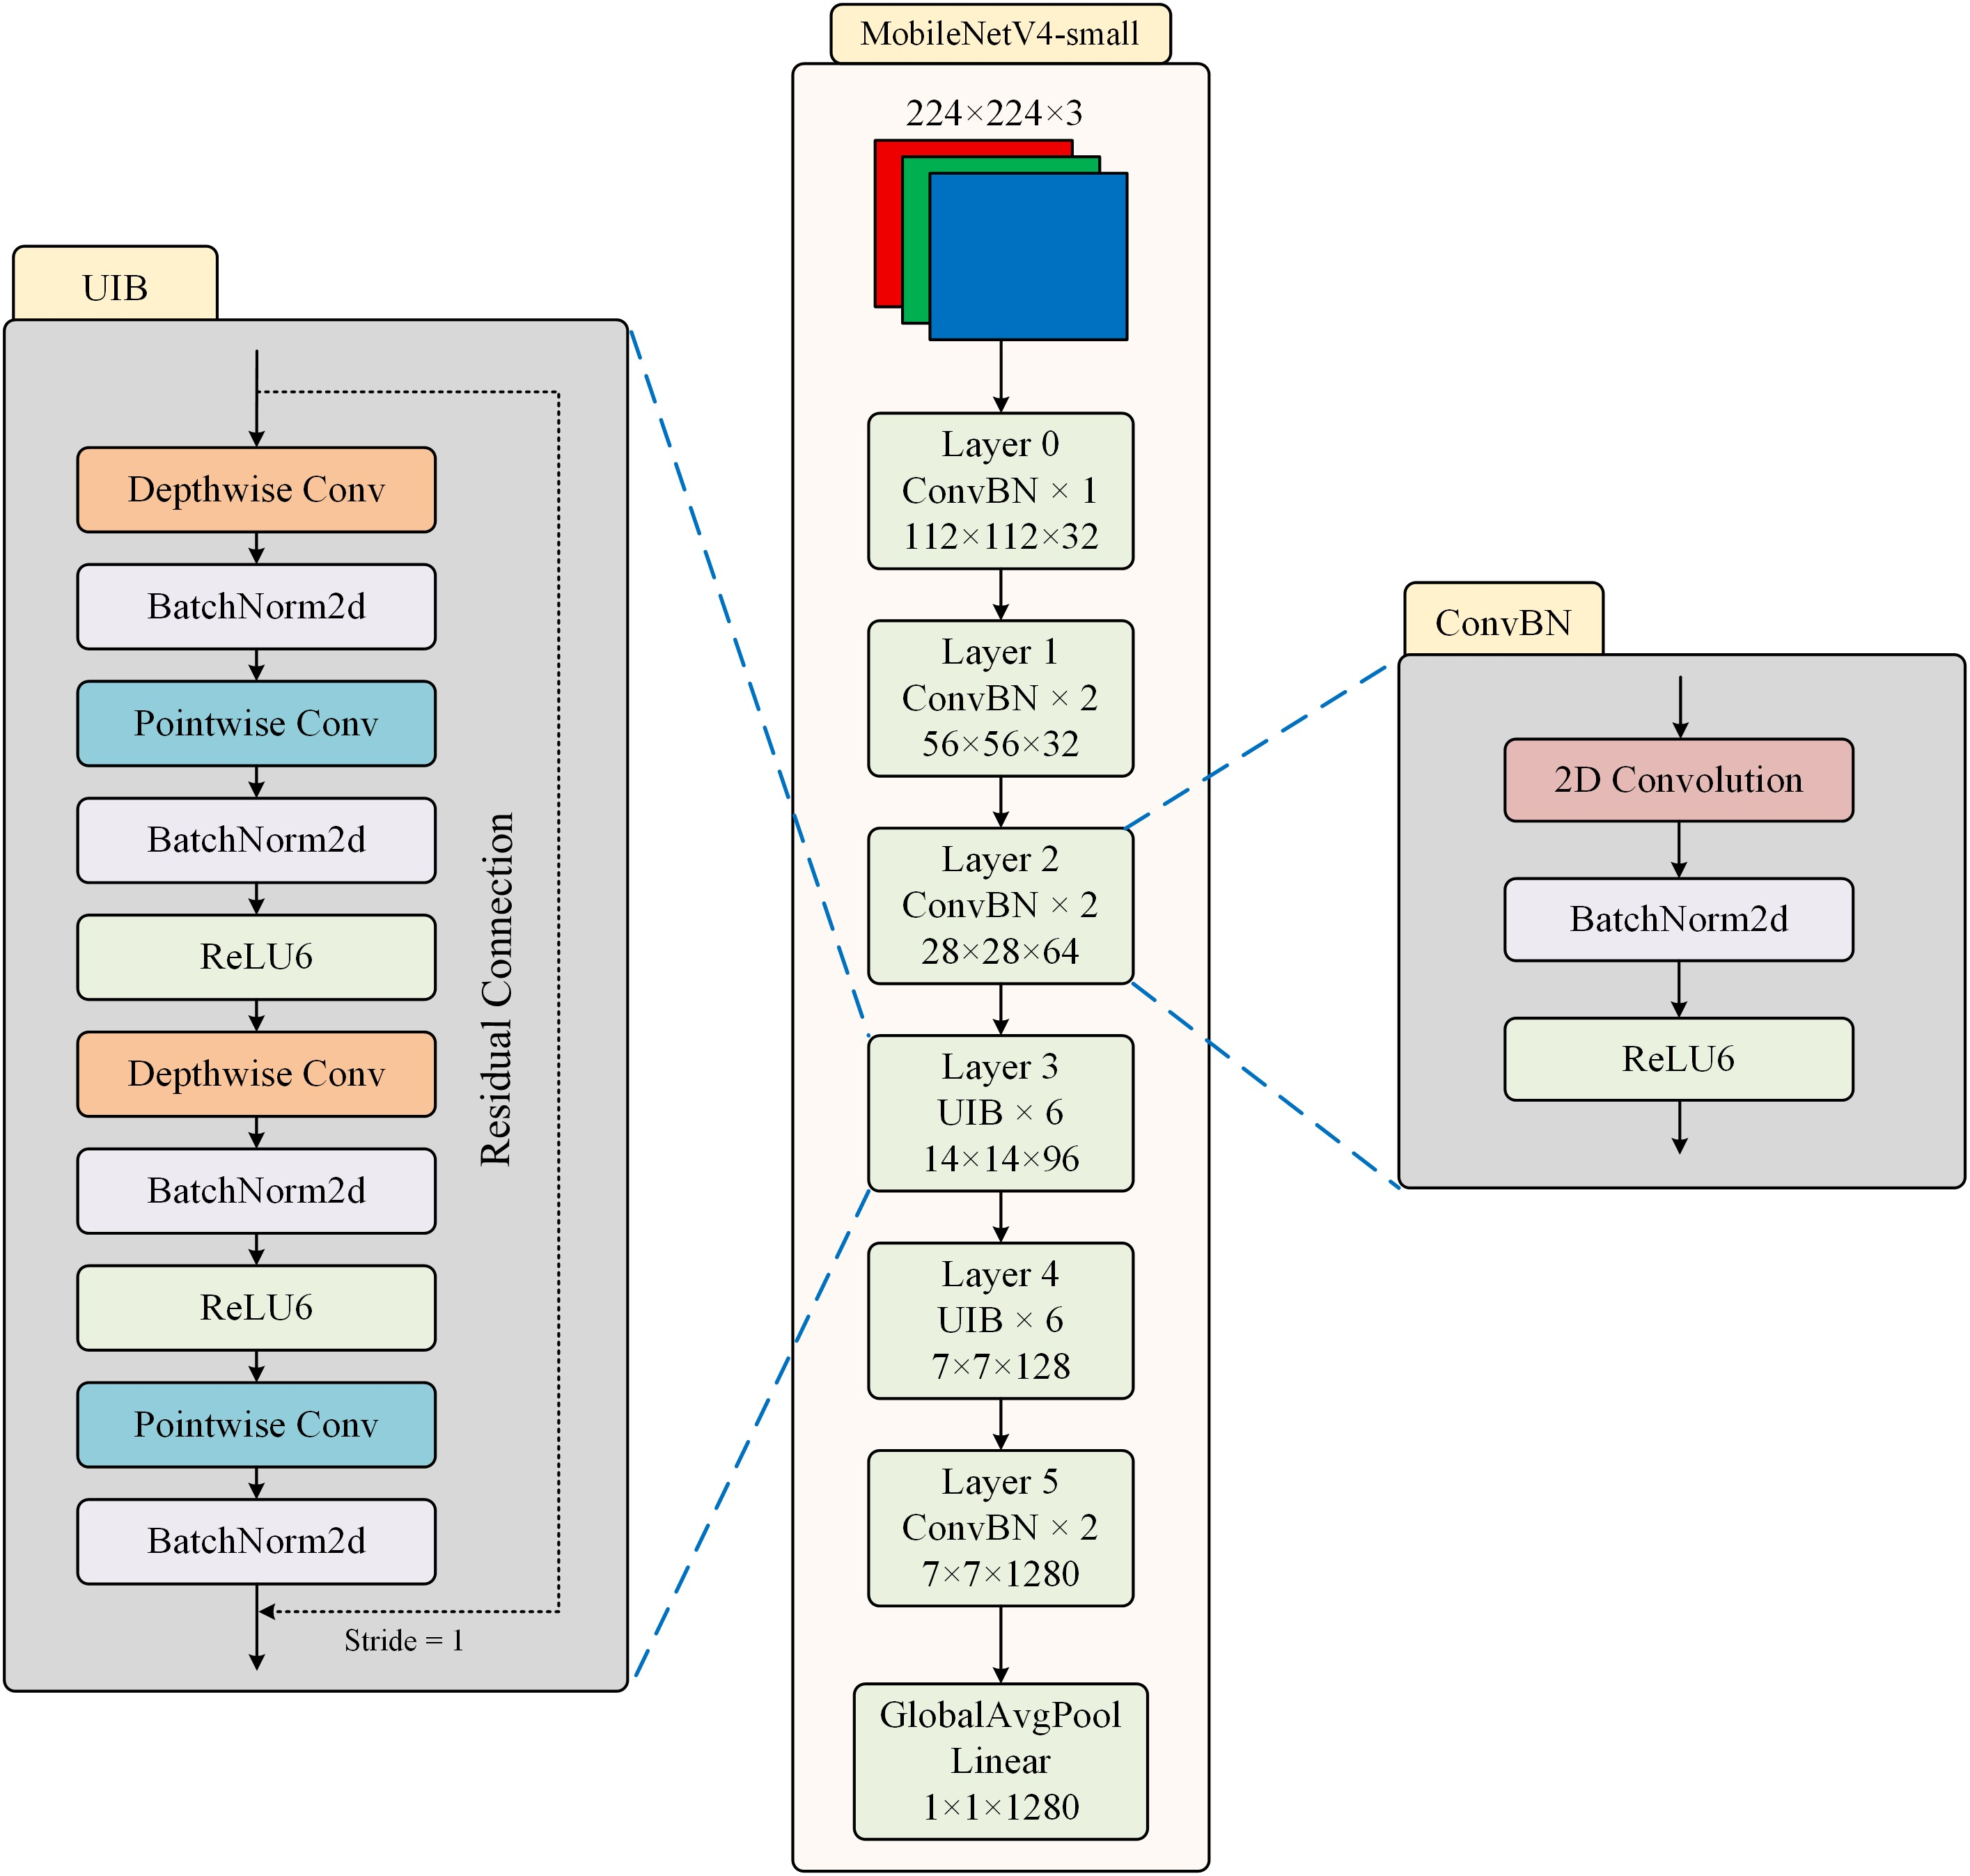
\includegraphics[width=1\linewidth]{Images/mobilenetv4.jpg}
%     \caption{A schematic overview of the MobileNetV4-small architecture \cite{chen_2025_mobilenetgdr}}
%     \label{fig:mbnv4}
% \end{figure}

% As shown in Figure \ref{fig:mbnv4}, the structure of MobileNetV4-Small is specifically optimized for extremely resource-constrained mobile and edge hardware. The architecture processes a standard $224 \times 224 \times 3$ input through a backbone of six layers (Layer 0–5), utilizing ConvBN blocks in the early and final stages and Universal Inverted Bottleneck (UIB) blocks in the deep stages to progressively downsample spatial resolution to $7 \times 7$. While the network adopts efficient depthwise separable convolution as its basic operation unit, it introduces a more flexible channel expansion mechanism compared to previous models. The UIB module dynamically adjusts the dilation rate of the convolution kernel, using a smaller receptive field in the shallow network to preserve detailed information and gradually expanding the receptive field in the deep network to capture global features. This adaptive mechanism significantly enhances the model’s adaptability to features of different scales. Furthermore, as illustrated in the UIB expansion detail, two optional Depthwise Convolutions (DWConv) are introduced within the inverted bottleneck block: one positioned before the expansion layer and the other between the expansion and compression layers. Additionally, an innovative dynamic channel adjustment mechanism allows the network to adaptively adjust the channel expansion ratio at each stage, enabling automatic optimization of feature processing strategies at different depths.

% \subsection{Implementing MobileNetV4 as Backbone of YOLO11}

% To address the computational constraints of edge devices while maintaining detection accuracy, we replaced the standard YOLOv11 backbone - typically composed of standard Convolutional (\texttt{Conv}) layers and Cross-Stage Partial (\texttt{C3K2}) blocks - with the lightweight MobileNetV4 architecture. This integration was achieved through a three-step process involving modular code implementation, task registration, and structural reconfiguration \cite{csdn_mobilenetv4}.

% \subsubsection{Modular Implementation of MobileNetV4}
% We first integrated the MobileNetV4 architecture into the codebase by creating a dedicated module, \texttt{mobilenetv4.py}, within the \texttt{ultralytics/nn/Addmodules} directory. This script defines the \texttt{MobileNetV4} class and its core components, specifically the Universal Inverted Bottleneck (UIB) blocks. The UIB is a flexible architectural unit that unifies Inverted Bottleneck (IB), ConvNext, and Feed-Forward Network (FFN) structures, allowing the model to adaptively select the most efficient operation for different network depths. We specifically implemented the \texttt{MobileNetV4ConvSmall} variant, which is optimized for mobile CPUs, using the configuration specs defined in \texttt{MNV4ConvSmall\_BLOCK\_SPECS} to ensure compatibility with the input resolution and channel widths of the detection head \cite{csdn_mobilenetv4}.

% \subsubsection{Task Registration and Forward Pass Modification}
% To enable the YOLOv11 system to recognize and execute the new backbone, we modified the core task management script (\texttt{ultralytics/nn/tasks.py}). This involved two key changes:
% \begin{itemize}
%     \item \textit{Module Registration:} We imported the \texttt{MobileNetV4ConvSmall} class and integrated it into the system to allow the parser to interpret the "MobileNetV4ConvSmall" string within the YAML configuration.
%     \item \textit{Forward Pass Adaptation:} We updated the \texttt{\_predict\_once} function to handle the specific output format of the MobileNetV4 backbone. Unlike the standard backbone which passes tensors sequentially, the MobileNetV4 module returns a list of features at different scales (P3, P4, P5). The modified logic extracts these multi-scale features correctly to feed them into the subsequent Neck and Head layers.
% \end{itemize}

% \subsubsection{Structural Reconfiguration (Replacing Conv and C3K2)}
% The final step involved redefining the model architecture using a custom YAML configuration file (\texttt{MobileNetV4.yaml}) placed in the \texttt{ultralytics/cfg/models/11/} directory. In the standard YOLOv11 architecture, the backbone consists of a sequence of \texttt{Conv} downsampling layers interspersed with \texttt{C3K2} feature extraction blocks. We completely removed these layers and replaced them with a single \texttt{MobileNetV4ConvSmall} module. This replacement significantly reduces the parameter count and floating-point operations (FLOPs) by leveraging the UIB's efficiency, while providing the necessary hierarchical feature maps required by the YOLOv11 detection head \cite{csdn_mobilenetv4}.


% \subsection{LiteRT Framework}
% To enable real-time inference in embedded environments, an efficient and lightweight inference framework is required. In this work, we adopt LiteRT (formerly known as TensorFlow Lite) \cite{googleaiedge_2024_github}, a deep learning runtime specifically designed for on-device machine learning under strict latency, memory, and power constraints. LiteRT has been widely used in embedded and edge systems due to its minimal runtime overhead and compatibility with optimized model representations. Recent studies on the sustainability of AI inference at the edge further emphasize that the choice of inference framework, together with model-level optimizations, plays a critical role in balancing accuracy, inference latency, and energy consumption on resource-constrained devices \cite{edge_sustainability_2025}. These considerations motivate the selection of LiteRT as the runtime engine for executing the proposed MobileNetV4-backed YOLO model.

% Unlike server-oriented deep learning frameworks that depend on dynamic memory allocation and complex runtime components, LiteRT employs a lightweight interpreter with a static memory allocation strategy. Its efficiency is largely enabled by the use of FlatBuffers, a compact serialization format that allows models to be memory-mapped directly without explicit parsing. This design significantly reduces both initialization overhead and memory footprint, making LiteRT well suited for embedded systems with limited computational and memory resources.

% Transitioning the trained YOLO11-MobileNetV4 model from the training environment to an embedded deployment target involves a two-step optimization process:
% \begin{itemize}
%     \item \textit{Conversion:} The trained model is converted into the \texttt{.tflite} format, during which graph-level optimizations such as operator fusion and constant folding are applied to streamline the computational graph.
%     \item \textit{Quantization:} To further reduce computational complexity and memory bandwidth requirements, Post-Training Quantization (PTQ) is applied. This process converts model weights from 32-bit floating-point (FP32) to 8-bit integers (INT8), substantially reducing the model size while preserving detection accuracy.
% \end{itemize}

% % \subsection{Implementing MobileNetV4 as Backbone of YOLO11}

% % To address the computational constraints of edge devices while maintaining detection accuracy, we replaced the standard YOLOv11 backbone - typically composed of standard Convolutional (\texttt{Conv}) layers and Cross-Stage Partial (\texttt{C3K2}) blocks - with the lightweight MobileNetV4 architecture. This integration was achieved through a three-step process involving modular code implementation, task registration, and structural reconfiguration \cite{csdn_mobilenetv4}.

% % \subsubsection{Modular Implementation of MobileNetV4}
% % We first integrated the MobileNetV4 architecture into the codebase by creating a dedicated module, \texttt{mobilenetv4.py}, within the \texttt{ultralytics/nn/Addmodules} directory. This script defines the \texttt{MobileNetV4} class and its core components, specifically the Universal Inverted Bottleneck (UIB) blocks. The UIB is a flexible architectural unit that unifies Inverted Bottleneck (IB), ConvNext, and Feed-Forward Network (FFN) structures, allowing the model to adaptively select the most efficient operation for different network depths. We specifically implemented the \texttt{MobileNetV4ConvSmall} variant, which is optimized for mobile CPUs, using the configuration specs defined in \texttt{MNV4ConvSmall\_BLOCK\_SPECS} to ensure compatibility with the input resolution and channel widths of the detection head \cite{csdn_mobilenetv4}.

% % \subsubsection{Task Registration and Forward Pass Modification}
% % To enable the YOLOv11 system to recognize and execute the new backbone, we modified the core task management script (\texttt{ultralytics/nn/tasks.py}). This involved two key changes:
% % \begin{itemize}
% %     \item \textit{Module Registration:} We imported the \texttt{MobileNetV4ConvSmall} class and integrated it into the system to allow the parser to interpret the "MobileNetV4ConvSmall" string within the YAML configuration.
% %     \item \textit{Forward Pass Adaptation:} We updated the \texttt{\_predict\_once} function to handle the specific output format of the MobileNetV4 backbone. Unlike the standard backbone which passes tensors sequentially, the MobileNetV4 module returns a list of features at different scales (P3, P4, P5). The modified logic extracts these multi-scale features correctly to feed them into the subsequent Neck and Head layers.
% % \end{itemize}

% % \subsubsection{Structural Reconfiguration (Replacing Conv and C3K2)}
% % The final step involved redefining the model architecture using a custom YAML configuration file (\texttt{MobileNetV4.yaml}) placed in the \texttt{ultralytics/cfg/models/11/} directory. In the standard YOLOv11 architecture, the backbone consists of a sequence of \texttt{Conv} downsampling layers interspersed with \texttt{C3K2} feature extraction blocks. We completely removed these layers and replaced them with a single \texttt{MobileNetV4ConvSmall} module. This replacement significantly reduces the parameter count and floating-point operations (FLOPs) by leveraging the UIB's efficiency, while providing the necessary hierarchical feature maps required by the YOLOv11 detection head \cite{csdn_mobilenetv4}.


% % -------------------------------New section---------------------------
% \section{Methodology: Hybrid YOLO--MobileNet Architecture for Edge Inference}
% \label{sec:yolo_mobilenet}

% Deploying deep learning-based object detection on resource constrained edge devices requires a balance between detection accuracy, computational efficiency, and deployment feasibility. To address these requirements, the proposed methodology combines a modern YOLO detection head with a lightweight MobileNetV4 backbone and an optimized on-device inference runtime. This hybrid design targets efficient CPU-based inference while preserving compatibility with embedded deployment constraints.

% \subsection{YOLO11 Detection Architecture}
% The YOLO (You Only Look Once) family is widely adopted for real-time object detection due to its end-to-end design and favorable accuracy-latency trade-offs \cite{ali_2024_the}. YOLO11, released in 2024, extends previous versions with architectural refinements that improve efficiency and task generality, supporting object detection, segmentation, and related vision tasks \cite{ultralytics_2024_yolo11}.

% \begin{figure}[htbp]
%     \centering
%     \resizebox{\columnwidth}{!}{%
%     \begin{tikzpicture}[
%         node distance=0.4cm and 0.8cm,
%         font=\sffamily\bfseries\small,
%         module/.style={
%             draw=cyan!60, fill=cyan!10, rounded corners, drop shadow,
%             minimum width=2.0cm, minimum height=0.8cm, align=center, line width=0.8pt, font=\scriptsize\sffamily\bfseries
%         },
%         yolo/.style={
%             draw=orange!60, fill=orange!10, rounded corners, drop shadow,
%             minimum width=2.2cm, minimum height=4.6cm, align=center, font=\sffamily\bfseries\normalsize
%         },
%         task/.style={
%             draw=green!60!black, fill=green!10, rounded corners, drop shadow,
%             minimum width=3.0cm, minimum height=0.6cm, align=center, anchor=west, line width=0.8pt, font=\scriptsize\sffamily\bfseries
%         },
%         line/.style={draw=gray!60, line width=1pt},
%         arrow/.style={line, -{Stealth[scale=1.0]}}
%     ]

%     % Central YOLOv11 block
%     \node[yolo] (yolo11) {YOLO11};

%     % Left-side modules (Three key modules)
%     % Position C2PSA to be aligned vertically with the center
%     \node[module, left=1.0cm of yolo11] (c2psa) {C2PSA};
%     \node[module, above=0.3cm of c2psa] (sppf) {SPPF};
%     \node[module, below=0.3cm of c2psa] (c3k2) {C3K2};

%     % Right-side tasks (6 tasks)
%     % Position the top task relative to the center, then stack others below
%     \node[task, right=1.0cm of yolo11, anchor=west, yshift=2.0cm] (od) {Object Detection};
%     \node[task, below=0.2cm of od] (is) {Instance Segmentation};
%     \node[task, below=0.2cm of is] (ic) {Image Classification};
%     \node[task, below=0.2cm of ic] (pe) {Pose Estimation};
%     \node[task, below=0.2cm of pe] (ood) {Oriented Object\\Detection};
%     \node[task, below=0.2cm of ood] (ot) {Object Tracking};

%     % Connections: Modules to YOLOv11
%     % Merge lines from the three modules
%     \coordinate (merge_x) at ($(c2psa.east)!0.5!(yolo11.west)$);
    
%     % Draw vertical bar connecting the top and bottom modules at merging x-coord
%     \draw[line] (sppf.east) -| (merge_x) |- (c3k2.east);
    
%     % Connect C2PSA to the merge point
%     \draw[line] (c2psa.east) -- (merge_x);
    
%     % Arrow from merge point to YOLOv11
%     % Since merge_x is a coordinate, we need the intersection with C2PSA's y-level
%     \draw[arrow] (merge_x |- c2psa.east) -- (yolo11.west);

%     % Connections: YOLOv11 to Tasks
%     % Draw arrows from the right edge of YOLOv11 to each task
%     \foreach \t in {od, is, ic, pe, ood, ot} {
%         \draw[arrow] (yolo11.east |- \t.west) -- (\t.west);
%     }

%     \end{tikzpicture}%
%     }
%     \caption{Key architectural modules in YOLO11.}
%     \label{fig:yolo11}
% \end{figure}

% Compared to YOLOv8, YOLO11 introduces optimized feature extraction modules such as Cross-Stage Partial with Self-Attention (C2PSA) and a lightweight CSP bottleneck variant (C3K2) in Figure \ref{fig:yolo11}, which enhance contextual feature representation while reducing computational overhead \cite{jegham_2025_yolo}. These characteristics make YOLO11 a suitable detection head for real-time perception when paired with an efficient backbone.

% \subsection{MobileNetV4 Backbone}
% MobileNetV4 is a lightweight convolutional neural network architecture introduced in 2024 to improve inference efficiency on mobile and edge computing platforms \cite{qin_2024_mobilenetv4}. Compared to earlier MobileNet variants, it provides a more favorable balance between inference latency and accuracy, making it suitable for real-time deployment on resource-constrained hardware \cite{chen_2025_mobilenetgdr}.

% In this work, we select the MobileNetV4-Small variant as the backbone of YOLO11 based primarily on its empirical inference efficiency on CPU-based platforms. As shown in Fig.~\ref{fig:mnv4_benchmark}, MobileNetV4 consistently achieves near-Pareto-optimal accuracy-latency trade-offs across diverse hardware backends, including general-purpose CPUs. At comparable latency levels, it outperforms previous MobileNet generations and competing lightweight architectures, which motivates its adoption for edge inference scenarios where low latency is a critical requirement \cite{qin_2024_mobilenetv4}.

% \begin{figure}[ht]
%     \centering
%     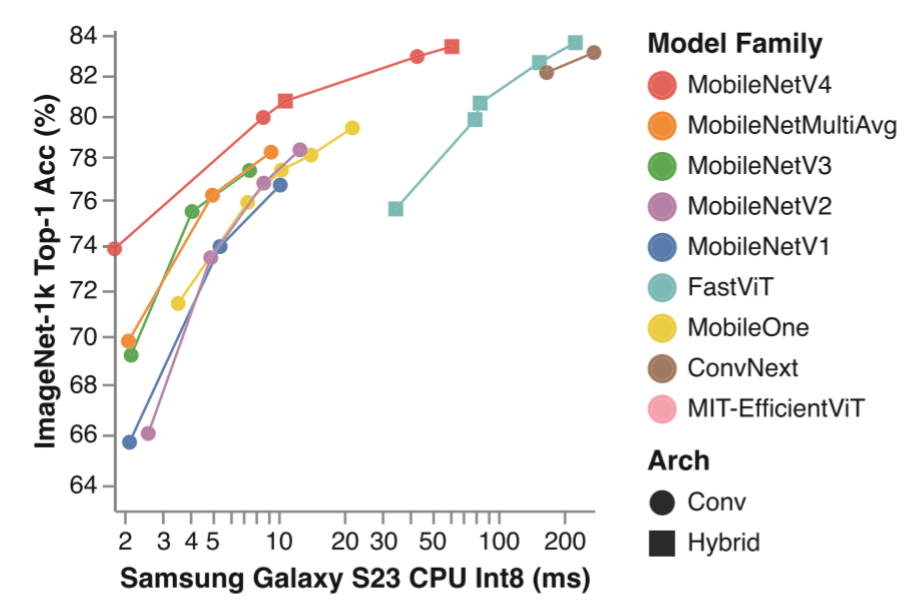
\includegraphics[width=1\linewidth]{Images/mnv4withothers.png}
%     \caption{MobileNetV4 models exhibit near-Pareto-optimal accuracy–latency trade-offs across multiple hardware platforms \cite{qin_2024_mobilenetv4}.}
%     \label{fig:mnv4_benchmark}
% \end{figure}


% % \subsection{YOLO11--MobileNetV4 Backbone Integration}
% % \label{subsec:yolo_mobilenetv4_integration}

% % To improve inference efficiency on resource-constrained devices, the standard YOLO11 backbone is replaced with the lightweight MobileNetV4-Small architecture. The original backbone, composed of convolutional and Cross-Stage Partial (CSP) blocks, introduces significant computational overhead, limiting real-time CPU execution. MobileNetV4 offers a more favorable accuracy-latency trade-off for embedded inference scenarios \cite{csdn_mobilenetv4}.

% % % The integration is performed at the framework and configuration level, following established practices in the Ultralytics YOLO ecosystem \cite{csdn_mobilenetv4}. The detection head remains unchanged, while the backbone is replaced to ensure that the extracted multi-scale feature maps remain compatible with the original YOLO11 neck and head.

% % % Algorithm~\ref{alg:yolo11_mobilenetv4} summarizes the backbone replacement procedure, including backbone removal, MobileNetV4-Small registration, feature map adaptation, and model validation.

% % % \begin{algorithm}[ht]
% % % \caption{YOLO11 Backbone Replacement with MobileNetV4-Small}
% % % \label{alg:yolo11_mobilenetv4}
% % % \begin{algorithmic}[1]
% % % \REQUIRE YOLO11 baseline model, MobileNetV4-Small definition
% % % \ENSURE YOLO11-MobileNetV4 detection model

% % % \STATE Remove the original YOLO11 backbone
% % % \STATE Register MobileNetV4-Small in the YOLO framework
% % % \STATE Configure multi-scale feature outputs
% % % \STATE Connect features to the YOLO neck and detection head
% % % \STATE Validate and export the integrated model

% % % \RETURN YOLO11-MobileNetV4 model
% % % \end{algorithmic}
% % % \end{algorithm}

% % % This substitution significantly reduces model complexity while preserving detection functionality, enabling real-time inference on CPU-based edge platforms.



% % % \subsection{Integrating MobileNetV4 as the YOLO11 Backbone}

% % % To optimize YOLO11 for deployment on resource-constrained edge devices, the standard backbone—traditionally comprised of standard Convolutional layers and Cross-Stage Partial (C3K2) blocks—was replaced with the MobileNetV4 architecture. This integration focuses on leveraging high-efficiency feature extraction to maintain a balance between detection precision and low-latency performance \cite{csdn_mobilenetv4}.

% % \subsubsection{Architectural Adaptation of MobileNetV4} The core of this integration involves the Universal Inverted Bottleneck (UIB) blocks, which are the hallmark of the MobileNetV4 design. The UIB serves as a unified structural unit that merges the advantages of Inverted Bottlenecks and ConvNext blocks, allowing for an adaptive computational flow across different network stages. For this implementation, the variant optimized for mobile CPUs was selected. This choice ensures that the spatial resolution and channel dimensions of the extracted features remain compatible with the multi-scale requirements of the YOLO11 detection head.

% % \subsubsection{Feature Alignment and Multi-Scale Fusion} A critical aspect of the integration involves adapting the model's forward pass logic to accommodate the specific output characteristics of MobileNetV4. While traditional backbones often process features through a linear sequence of layers, the MobileNetV4 module is configured to provide a hierarchical set of feature maps (P3, P4, and P5) simultaneously. The system architecture was modified to parse these multi-scale features directly, ensuring a seamless transition of data from the lightweight backbone into the Neck and Head components for final bounding box regression and classification.

% % \subsubsection{Structural Optimization and Complexity Reduction} The final architectural transition involves the wholesale replacement of the original YOLO11 feature extraction sequence with the MobileNetV4 framework. By removing the computationally intensive C3K2 blocks and standard downsampling convolutions, the model significantly reduces its total parameter count and floating-point operations (FLOPs). This structural reconfiguration allows the network to benefit from the UIB’s efficiency while retaining the essential hierarchical feature representation necessary for robust object detection in diverse environments \cite{csdn_mobilenetv4}.


% \subsection{YOLO11--MobileNetV4 Backbone Integration}
% \label{subsec:yolo_mobilenetv4_integration}

% To adapt YOLO11 for efficient inference on CPU-based and resource-constrained edge devices, the original backbone is replaced with the lightweight MobileNetV4-Small architecture. The integration is implemented following the modular design of the Ultralytics YOLO framework, where backbone, neck, and detection head are decoupled and independently configurable.

% First, the MobileNetV4 backbone is added to the YOLO codebase as a custom module. A new directory is created under \texttt{ultralytics/nn}, and the MobileNetV4 implementation-including Universal Inverted Bottleneck (UIB) blocks and predefined block specifications-is placed in a dedicated \texttt{mobilenetv4.py} file. This module encapsulates all backbone variants (Small, Medium, and Large) and exposes intermediate feature stages required for detection \cite{csdn_mobilenetv4}.

% Next, the YOLO model construction logic is extended by modifying \texttt{ultralytics/nn/tasks.py} to register the MobileNetV4 backbone. This step enables the framework to correctly instantiate the new backbone, parse its layer definitions, and integrate it into the standard YOLO forward pass.

% Finally, a custom model configuration file (YAML) is created to define the YOLO11–MobileNetV4 architecture. In this configuration, the original YOLO11 backbone (C3k2 and Conv) is replaced with MobileNetV4-Small, while the neck and detection head remain unchanged. The backbone is configured to output three multi-scale feature maps corresponding to P3, P4, and P5, which are directly routed to the YOLO neck for feature fusion and detection.

% By adding these modules and configuration files, the original YOLO11 backbone can be seamlessly substituted with MobileNetV4 without altering the detection head or loss functions. This replacement significantly reduces model complexity and computational cost while preserving the multi-scale detection capability of YOLO11, enabling efficient inference on embedded edge platforms.




% \subsection{LiteRT Inference Framework}
% Efficient on-device inference further requires a lightweight runtime optimized for embedded environments. The proposed system employs LiteRT (formerly TensorFlow Lite) \cite{googleaiedge_2024_github}, a deep learning runtime designed for low-latency and low-memory execution. LiteRT uses a lightweight interpreter and static memory allocation, enabled by FlatBuffers-based model serialization, which minimizes initialization overhead and runtime footprint.

% Recent studies on edge AI sustainability highlight that runtime selection and model quantization are critical factors in balancing inference latency, accuracy, and energy consumption on constrained devices~\cite{edge_sustainability_2025}. Accordingly, the trained YOLO11-MobileNetV4 model is converted to the \texttt{.tflite} format and optimized using post-training quantization. This approach aligns with TinyML principles, where quantized convolutional networks are deployed on resource-constrained platforms, as demonstrated in recent object classification systems~\cite{10636597}. The applied optimization reduces model size and computational complexity while maintaining detection performance, enabling efficient CPU-only deployment in embedded environments.



%--------------------------New New Section------------------------
\section{Methodology: Hybrid YOLO--MobileNet Architecture for Edge Inference}
\label{sec:yolo_mobilenet}

Deploying deep learning--based object detection on resource-constrained edge devices requires balancing detection accuracy and computational efficiency. To address this challenge, the proposed methodology combines a YOLO detection head with a lightweight MobileNetV4 backbone and an optimized on-device inference pipeline, targeting efficient CPU-based deployment on embedded platforms.

\subsection{YOLO--MobileNetV4}
This subsection presents the hybrid YOLO--MobileNetV4 design for CPU-centric edge inference, including the MobileNetV4 backbone, the motivation for its integration with YOLO, and a concise backbone-replacement procedure within the Ultralytics framework.

\subsubsection{MobileNetV4}
MobileNetV4 demonstrates strong suitability for CPU-based edge devices due to its favorable accuracy--latency trade-offs on general-purpose processors. As shown in Fig.~\ref{fig:mnv4_benchmark}, MobileNetV4 consistently achieves near--Pareto-optimal performance on mobile CPUs (e.g., Galaxy~S23), outperforming earlier MobileNet variants at comparable latency. Its Universal Inverted Bottleneck (UIB) design enables efficient integer arithmetic and regular memory access, making MobileNetV4-Small well suited for real-time inference under strict latency and power constraints \cite{qin_2024_mobilenetv4}. These efficiency characteristics motivate the integration of MobileNetV4 into the YOLO framework, one of the most widely adopted architectures for practical sensor-class deployment.

\begin{figure}[ht]
    \centering
    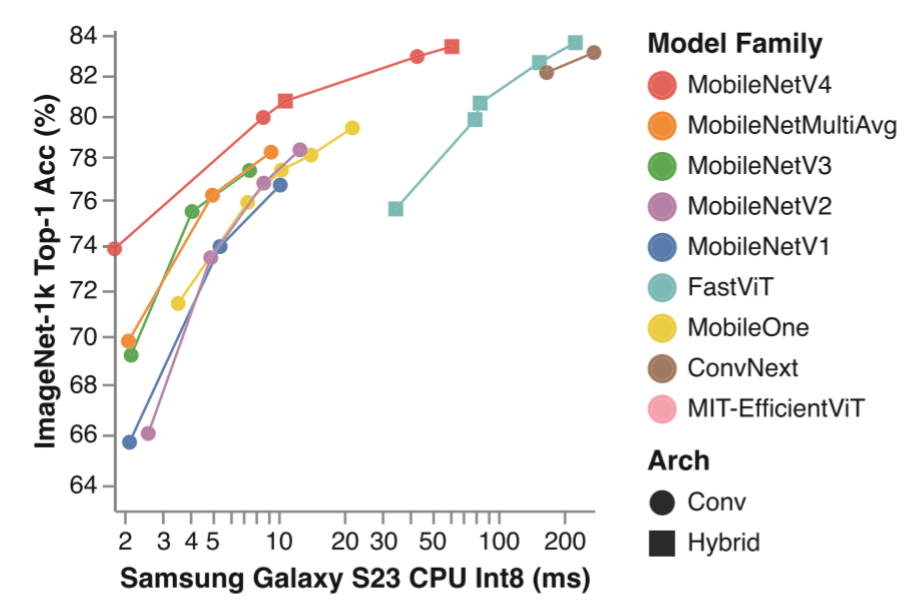
\includegraphics[width=0.9\linewidth]{Images/mnv4withothers.png}
    \caption{MobileNetV4 models exhibit near-Pareto-optimal accuracy--latency trade-offs on Samsung~S23 device \cite{qin_2024_mobilenetv4}.}
    \label{fig:mnv4_benchmark}
\end{figure}

\subsubsection{YOLO--MobileNetV4 Integration for Sensor-Class Devices}
The YOLO family is widely adopted for real-time object detection due to its efficient heads and multi-scale design \cite{lei2025emnv4}\cite{ qin_2024_mobilenetv4}\cite{chen_2025_mobilenetgdr}. However, conventional YOLO backbones based on CSP/C3 blocks are computationally intensive and unsuitable for CPU-only sensor-class devices. To enable efficient embedded inference, the original YOLO11 backbone is replaced with MobileNetV4, preserving multi-scale detection while significantly reducing computational cost.

The integration follows the modular design of the Ultralytics YOLO framework, where backbone, neck, and detection head are decoupled. In summary, MobileNetV4 is implemented as a custom backbone module (\texttt{ultralytics/nn/mobilenetv4.py}) exposing P3--P5 feature maps, registered in the model factory (\texttt{ultralytics/nn/tasks.py}), and aligned with the YOLO neck using lightweight $1\times1$ adapters when required. A custom YAML configuration (\texttt{yolo11\_mnv4.yaml}) replaces the original C3k2/Conv backbone with MobileNetV4-ConvSmall, and the integrated model is validated prior to ONNX and TFLite export.


\subsection{Implementation: YOLO--MobileNetV4 on LiteRT}
\label{subsec:impl_litert_cpp}

To enable efficient CPU-only inference on sensor-class edge devices, this work adopts LiteRT (formerly TensorFlow Lite) and implements the complete inference pipeline in C++ to minimize runtime overhead and reduce CPU inference latency. Unlike common Python-based deployments, the proposed C++ implementation leverages LiteRT’s static tensor allocation and FlatBuffers-based model serialization to achieve deterministic and low-memory execution. In accordance with edge AI sustainability principles \cite{11214219}, the YOLO11--MobileNetV4 model is converted to the \texttt{.tflite} format and optimized via post-training quantization, enabling efficient deployment without dedicated accelerators. To the best of our knowledge, this work represents one of the first end-to-end implementations that combines a YOLO11--MobileNetV4 detector with a fully C++ LiteRT runtime for real-time inference on CPU-based sensor devices. The overall inference workflow is summarized in Algorithm~\ref{alg:litert_yolo_mnv4}.


\begin{algorithm}[ht]
\caption{LiteRT-based YOLO11--MobileNetV4 Inference Pipeline}
\label{alg:litert_yolo_mnv4}
\begin{algorithmic}[1]
\REQUIRE Input frame $I$, LiteRT model $M$
\ENSURE Final detections $\mathcal{D}$

\STATE // --- Initialization ---
\STATE Load \texttt{.tflite} model $M$
\STATE Create LiteRT interpreter and allocate static tensors
\STATE Configure CPU threads for inference

\STATE // --- Preprocessing ---
\STATE Compute letterbox scale and padding
\STATE Resize $I$ and pad to network input size
\STATE Convert color space and normalize pixel values
\STATE Copy preprocessed data to input tensor

\STATE // --- Inference ---
\STATE Invoke LiteRT interpreter forward pass

\STATE // --- Postprocessing ---
\FOR{each prediction $p$ in output tensor}
    \STATE Decode bounding box and confidence score
    \STATE Discard $p$ if confidence $< \tau_c$
    \STATE Map box coordinates back to original image space
    \STATE Append valid detection to proposal set
\ENDFOR

\STATE Apply class-wise Non-Maximum Suppression with threshold $\tau_{iou}$

\STATE // --- Output ---
\STATE Encode final detections and publish to sensor interface
\RETURN $\mathcal{D}$
\end{algorithmic}
\end{algorithm}

Although the proposed YOLO--MobileNetV4 architecture enables efficient edge inference, its practical deployment in automotive systems requires a standardized and safety-aware software framework. The following section therefore introduces the AUTOSAR Adaptive Platform and discusses its role in supporting efficient and reliable execution of edge AI perception services.



